\documentclass[10pt,a4paper]{article}
\usepackage[top=2cm, bottom= 2cm, left=2cm, right=2cm]{geometry}
\usepackage[utf8]{inputenc}
\usepackage[T1]{fontenc}
\usepackage{amsmath}
\usepackage{amssymb}
\usepackage{float}
\usepackage{makeidx}
\usepackage{graphicx}
\usepackage{siunitx}
\usepackage{hyperref}
\usepackage{mathtools}
\usepackage[portuguese]{babel}


\hypersetup{
hidelinks = true
}

\author{Arthur de Souza Molina e Gabriel Capelini Magalhaes}
\title{Resolução da primeira prova de Física Moderna 1 A}
\begin{document}
	\maketitle
	
	\begin{enumerate}
	\item Considere o seguinte conjunto de matrizes $\Lambda$: 
	\begin{equation} \label{metrica}
	\Lambda^{T} \eta \Lambda = \eta \Rightarrow \Lambda \in O(3,1)
	\end{equation}
	
	onde $\eta$ é a métrica do espaço de Minkowsky. 
	\begin{enumerate}
	\item Determine os possíveis valores para o determinante de $\Lambda$
	\paragraph{Solução:} Tomando o determinante de ambos os lados de (\ref{metrica}), temos 
	
	\begin{equation}
\begin{split}
	&\text{det}(\Lambda^{T} \eta \Lambda) = \det(\eta) \Rightarrow \text{det}(\Lambda^{T})\text{det}(\eta)\text{det}(\Lambda) = \det(\eta)\Rightarrow \text{det}(\Lambda^{T})\text{det}(\Lambda) = 1 \\ 
	&\Rightarrow (\text{det}(\Lambda))^2 = 1 \Rightarrow \text{det}(\Lambda) = \pm 1	
	\end{split}
	\end{equation}
	
	onde foi usado $\text{det}(\Lambda^T) = \text{det}(\Lambda)$ e $\text{det}(\eta) = -1$.
	\item O subconjunto
	\begin{equation} \label{det negativo}
	\Lambda \in O(3,1) \quad \text{com} \quad \text{det }\Lambda = -1
	\end{equation}
	forma um grupo?
	
	\paragraph{Solução:} Vamos checar as propriedades de grupos para verificar se (\ref{det negativo}) forma um grupo
	\begin{enumerate}
	\item Fechado 
	
	Sejam duas matrizes $\Lambda$ e $\Lambda'$ em que $\text{det}\Lambda = \text{det}\Lambda' = -1$. Temos então que 
	\begin{equation}
	\Lambda \cdot \Lambda' = \Lambda'' \Rightarrow \text{det}(\Lambda \cdot \Lambda') = \text{det}(\Lambda''	) \Rightarrow \text{det}(\Lambda)\cdot \text{det}(\Lambda') = \text{det}(\Lambda'') \Rightarrow \text{det}(\Lambda'') = 1
	\end{equation}
	
	Portanto, veja que o produto de duas matrizes de determinante igual a -1 nos dá uma matriz com determinante igual a 1. Porém, de (\ref{det negativo}) temos que esse subconjunto são todas as matrizes com determinante igual a -1. Logo o produto de duas matrizes pertencentes a (\ref{det negativo}) não produz uma matriz que pertence a (\ref{det negativo}). Portanto não pode formar um grupo.
	\end{enumerate}
	\end{enumerate}
	
	\item Escreva a matriz $\Lambda$ para uma transformação de Lorentz (um boost) com velocidade 
	\begin{equation}\label{velocidade arbitrária}
	\mathbf{v} = \frac{b\sqrt{3}}{2}\mathbf{\hat{y}}-\frac{b}{2}\mathbf{\hat{z}}, \;\; b = \text{ constante}
	\end{equation}
	
	\paragraph{Solução:} Como esse boost tem uma direção arbitrária, é necessário aplicarmos uma rotação para alinhar os eixos. Pela velocidade só ter componentes em $\mathbf{\hat{y}}$ e $\mathbf{\hat{z}}$, podemos tratar esse problema como bidimensional (por conveniência). A seguir está representado esquematicamente a situação 
	
	\begin{figure}[H]
	\centering
	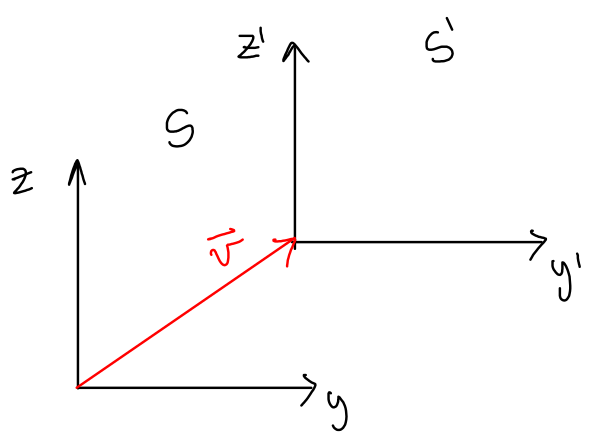
\includegraphics[scale=0.30]{figuras/boost.png}
	\caption{Movimento entre dois referenciais para uma velocidade igual a (\ref{velocidade arbitrária}).}
	\end{figure}
	
	A partir dessa figura, é fácil ver que se rotacionarmos os referenciais em torno de $x$ de um ângulo $\theta$ (que pode ser encontrado mais tarde), alinhamos o eixo $y$ com a direção da velocidade e então podemos aplicar a matriz e boost para $y$, dada por 
	
\begin{equation} 
\tilde{\Lambda}=\begin{pmatrix}
\gamma & 0 & -\gamma \beta & 0 \\ 
0 & 1 & 0 & 0 \\ 
-\gamma \beta & 0 & \gamma & 0 \\ 
0 & 0 & 0 & 1
\end{pmatrix} 
\end{equation}

A matriz de rotação em torno de $x$ é dada por 

\begin{equation}
R_{(x)}=\begin{pmatrix}
1 & 0 & 0 & 0 \\ 
0 & 1 & 0 & 0 \\ 
0 & 0 & \cos\theta & \sin\theta \\ 
0 & 0 & -\sin\theta & \cos\theta
\end{pmatrix} 
\end{equation}

Como $R_{(x)} \in SO(3)$, então $R^{-1} = R^T$. Então

\begin{equation}
R_{(x)}^{-1}=\begin{pmatrix}
1 & 0 & 0 & 0 \\ 
0 & 1 & 0 & 0 \\ 
0 & 0 & \cos\theta & -\sin\theta \\ 
0 & 0 & \sin\theta & \cos\theta
\end{pmatrix} 
\end{equation}

Portanto, a matriz que faz esse boost é dada por 

\begin{equation} \label{boost arbitrário}
\begin{split}
&\Lambda = R_{(x)}^{-1}\tilde{\Lambda}R_{(x)} = \begin{pmatrix}
1 & 0 & 0 & 0 \\ 
0 & 1 & 0 & 0 \\ 
0 & 0 & \cos\theta & -\sin\theta \\ 
0 & 0 & \sin\theta & \cos\theta
\end{pmatrix} 
\begin{pmatrix}
\gamma & 0 & -\gamma \beta & 0 \\ 
0 & 1 & 0 & 0 \\ 
-\gamma \beta & 0 & \gamma & 0 \\ 
0 & 0 & 0 & 1
\end{pmatrix} \begin{pmatrix}
1 & 0 & 0 & 0 \\ 
0 & 1 & 0 & 0 \\ 
0 & 0 & \cos\theta & \sin\theta \\ 
0 & 0 & -\sin\theta & \cos\theta
\end{pmatrix} \\
&= \begin{pmatrix}
\gamma & 0 &  -\gamma \beta & 0 \\ 
0 & 1 & 0 & 0 \\ 
-\gamma \beta \cos\theta & 0 & \beta\cos\theta & -\sin\theta \\ 
-\gamma \beta \sin\theta & 0 & \beta \sin\theta & \cos\theta
\end{pmatrix} \begin{pmatrix}
1 & 0 & 0 & 0 \\ 
0 & 1 & 0 & 0 \\ 
0 & 0 & \cos\theta & \sin\theta \\ 
0 & 0 & -\sin\theta & \cos\theta
\end{pmatrix} \\
&= \begin{pmatrix}
\gamma & 0 & -\gamma \beta \cos\theta & -\gamma \beta \sin\theta \\ 
0 & 1 & 0 & 0 \\ 
-\gamma \beta \cos\theta & 0 & \beta cos^2\theta + \sin^2\theta & \beta \cos\theta \sin\theta-\cos\theta \sin\theta \\ 
-\gamma \beta \sin\theta & 0 & \beta\cos\theta \sin\theta - \cos\theta \sin\theta & \beta \sin^2\theta + \cos^2\theta
\end{pmatrix} 
\end{split}
\end{equation}

De (\ref{velocidade arbitrária}) temos 

\begin{equation}
v = \sqrt{\frac{3b^2}{4}+\frac{b^2}{4}} = b
\end{equation}

Logo, tomando a projeção de $\mathbf{v}$ na direção de $\mathbf{\hat{y}}$, temos 

\begin{equation}
\mathbf{v}\cdot\mathbf{\hat{y}} = vy\cos\theta \Rightarrow \cos\theta = \frac{\frac{\sqrt{3}b}{2} }{b} = \frac{\sqrt{3}}{2}
\end{equation}

Portanto 

\begin{equation}
\theta = \arccos\left(\frac{\sqrt{3}}{2}\right) = \frac{\pi}{6}
\end{equation}
	
	
Substituindo esse valor em (\ref{boost arbitrário}) teremos a matriz que faz esse boost.
	\item Considere um túnel (reto e muito longo). O comprimento próprio do túnel (ou seja, medido por um observador parado com o túnel) vale L. Fixo na entrada do túnel temos um relógio, que vamos chamar de $R_1$, e outro relógio fixo na saída do túnel, que vamos chamar de $R_2$. Os relógios $R_1$ e $R_2$ estão perfeitamente sincronizados no referencial do túnel (i.e., num referencial onde o túnel está parado). Considere agora um carro (muito rápido) que entra no túnel. O piloto do carro também possui um relógio (ou seja, um relógio que anda junto com o carro). Quando o carro entrou no túnel tanto o relógio do piloto, quanto o relógio $R_1$ (o da entrada do túnel) marcavam um tempo igual a zero. Sabendo que, no instante em que o carro saiu do túnel, o relógio do piloto marcava um tempo
	
	\begin{equation}
	T = \frac{2L}{c}
	\end{equation}
	
	quanto marcava o relógio $R_2$ (o da saída do túnel) neste instante?
	
	\textbf{Solução:}
	
	Considerando $ R_1 $ e $ R_2 $ parados no referencial S e o carro parado com o relógio $ R_3 $ no referencial S', temos as seguintes relações:
	
	O relógio $ R_1 $ está sincronizado perfeitamente com o relógio $ R_2 $, em outras palavras, $ \Delta t_{R_1} = \Delta t_{R_2}$.
	
	O instante inicial do relógio $ R_1 $ é igual ao instante inicial do relógio $ R_3 $ e é zero, isto é, $ t_{R_1I} = t_{R_3I} = 0  $
	
	Usando uma das transformações de Lorentz, temos
	
	\begin{equation*}
		\Delta t' = \gamma ( \Delta t - \frac{v \Delta x}{c^2})
	\end{equation*}
	logo,
	\begin{equation*}
		\Delta t_{R_3} = \gamma ( \Delta t_{R_2} - \dfrac{v \Delta x}{c^2})
	\end{equation*}

	\begin{equation*}
		\therefore \,\,\,\Delta t_{R_2} =  ( \dfrac{\Delta t_{R_3}}{\gamma} + \dfrac{v \Delta x}{c^2})
	\end{equation*}

	\begin{equation*}
		\Delta t_{R_2} =  ( \dfrac{\dfrac{2L}{c}}{\gamma} + \dfrac{v L}{c^2}) = \dfrac{2L}{c\gamma} + \frac{vL}{c^2} = L (\dfrac{2}{c\gamma} + \dfrac{v}{c^2}) = \dfrac{L}{c} (\dfrac{2}{\gamma} + \dfrac{v}{c})
	\end{equation*}

	Sabendo que $ \Delta t_{R_3} = \dfrac{2L}{c} $ e a distância percorrida pelo piloto $ \Delta x\prime = \dfrac{\Delta x}{\gamma} = \dfrac{L}{\gamma} $, podemos calcular a velocidade
	
	\begin{equation*}
		v = \dfrac{\Delta x\prime}{\Delta t\prime} = \dfrac{\dfrac{L}{\gamma}}{\dfrac{2L}{c}} = \dfrac{c}{2\gamma}
	\end{equation*}

	\begin{equation*}
		v^2 = (\dfrac{c}{2\gamma})^2 = \dfrac{c^2}{4\gamma^2} = (\dfrac{c^2}{4}) (1 - \dfrac{v^2}{c^2})
	\end{equation*}

	\begin{equation*}
		v^2 + \dfrac{v^2}{4}= \dfrac{5v^2}{4}=  \dfrac{c^2}{4}
	\end{equation*}
	
	\begin{equation*}
	 \therefore	\,\,\,\, v  = \dfrac{c}{\sqrt{5}} < c
	\end{equation*}

	Calculando o $ \gamma $, temos
	
	\begin{equation*}
		\gamma = (1-\dfrac{v^2}{c^2})^{-1/2} = (1-\dfrac{(\dfrac{c}{\sqrt{5}})^2}{c^2})^{-1/2} =(1-\dfrac{1}{5})^{-1/2} = (\dfrac{4}{5})^{-1/2} = \dfrac{\sqrt{5}}{2}
	\end{equation*}

	\begin{equation*}
		\gamma = \dfrac{\sqrt{5}}{2} > 1
	\end{equation*}
	
	Substituindo o valor de $ v $ e $ \gamma $, obtemos
	
	\begin{equation*}
		\Delta t_{R_2}  = \dfrac{L}{c} (\dfrac{2}{\gamma} + \dfrac{v}{c}) = \dfrac{L}{c} (\dfrac{2}{ \dfrac{\sqrt{5}}{2}} + \dfrac{\dfrac{c}{\sqrt{5}}}{c})
	\end{equation*}

	\begin{equation*}
		\Delta t_{R_2}  = \dfrac{5L}{c\sqrt{5}} = \dfrac{L\sqrt{5}}{c}
	\end{equation*}

	O relógio $ R_2 $ marca $\dfrac{L\sqrt{5}}{c}  $ neste instante.
	
	\item Considere um fio onde corre uma corrente $I$. No referencial do laboratório, que vamos chamar de $S$, o fio está parado, possui uma densidade de carga $\rho$ (i.e, o fio \textbf{não é neutro}) e se estende reto paralelo ao eixo y. Ainda para esse referencial $S$, os elétrons responsáveis pela corrente se deslocam pelo fio com velocidade constante $\mathbf{v} =v \mathbf{\hat{y}}$. Considere também um outro referencial S que se desloca com relação à S, com velocidade $\mathbf{V} = \mathbf{v} = v\mathbf{\hat{y}}$
	\begin{enumerate}
		\item Determine os campos elétricos e magnéticos nos referenciais $S$ e $\tilde{S}$
		
		\textbf{Solução: }
		
		No referencial $ S $, temos os elétrons se movendo com velocidade constante $\mathbf{v} =v \mathbf{\hat{y}}$ e o fio carregado com a densidade de carga $\rho$. Portanto,
		
		ao usar a Lei de Gauss para determinar o campo elétrico produzido pelo fio, temos
		\begin{equation*}
			E = \dfrac{\rho l}{2\pi \epsilon_0s^2 }\vec{s}
		\end{equation*}
		onde l é o comprimento do fio e calculando o campo elétrico produzido pela carga
		\begin{equation*}
			E = \dfrac{-q}{4\pi \epsilon_0 r^3}\vec{r}
		\end{equation*}
		O campo elétrico total visto no referencial S é
		\begin{equation*}
			E = \dfrac{\rho l}{2\pi \epsilon_0s }\vec{s}-\dfrac{q}{4\pi \epsilon_0 r^3}\vec{r}
		\end{equation*}
		O campo magnético toal visto no referencial S é
		\begin{equation*}
			B = \dfrac{\mu_0 I}{2\pi s^3}\vec{s} 
		\end{equation*}
		pois é produzido pela corrente I do fio.
		
		No referencial $\tilde{S}$, temos
		
		o campo elétrico eletrostático gerado pelos elétrons do fio
		\begin{equation*}
			E = \dfrac{-q}{4\pi \epsilon_0 r^3}\vec{r}
		\end{equation*}
		Ao analisarmos a densidade de carga do fio no referencial $\tilde{S}$, é preciso ter cuidado, a relação da densidade de carga positiva e negativa do fio é dada por
		\begin{equation*}
			\rho_+ +\rho_- = \rho
		\end{equation*}
		onde
		\begin{equation*}
			\rho_+ = \frac{Q_+}{l}\text{ e  } \rho_- = \frac{Q_-}{l}
		\end{equation*}
		no referencial $ S $.
		Para $\tilde{S}$, a distância entre os elétrons é maior em comparação a distância entre os elétrons medida por um observador no referencial $ S $, logo a densidade de carga negativa é dada por
		\begin{equation*}
			\rho_-'  = \dfrac{Q_-}{l'}=\dfrac{Q_-}{\gamma l} = \gamma^{-1} \rho_-
		\end{equation*}
		Para um observador no referencial $\tilde{S}$ o fio é contraído, logo
		\begin{equation*}
			\rho_+\prime = \dfrac{Q_+}{l\prime} = \dfrac{Q_+}{\dfrac{l}{\gamma}} = \gamma\rho_+
		\end{equation*}
		portanto, a densidade de carga $\rho\prime$ observada em $\tilde{S}$ é observada com uma concentração maior de densidade de carga positiva, isto é,
		\begin{equation*}
			\rho\prime = \gamma\rho_+ + \gamma^{-1}\rho_- > \rho = \rho_+ + \rho_-
		\end{equation*}
		O campo elétrico gerado pelo fio é dado por
		\begin{equation*}
			E' = \dfrac{l\rho\prime }{2\pi \epsilon_0s^2 }\vec{s}
		\end{equation*}
		onde $ E'_{fio} > E_{fio} $.
		Neste referencial, a carga está em repouso e quem se move é o fio em sentido contrário, portanto, surge um campo magnético produzida pelo fio. A corrente elétrica e a carga pode ser reescrita como 
		\begin{equation*}
			i = \dfrac{dq}{dt} = \dfrac{dl}{dt}\dfrac{dq}{dl} = v \dfrac{dq}{dl}
		\end{equation*}
		e a densidade de carga
		\begin{equation*}
			dq = \rho dl \Rightarrow \dfrac{dq}{dl} = \rho
		\end{equation*}
		logo,
		\begin{equation*}
			i = v\dfrac{dq}{dl} = v\rho
		\end{equation*}	
		então
		\begin{equation*}
			B'_{fio} = \dfrac{\mu_0 i\prime}{2\pi s^2}\vec{s} = \dfrac{\mu_0 v\rho\prime}{2\pi s^2}\vec{s}
		\end{equation*}
		
		\item Considere agora uma carga q a uma distância $R$ do fio. A carga está parada com relação ao referencial $S$ (o laboratório). Determine as forças que agem na carga $q$ quando medidas por observadores nos referenciais $S$ e $\tilde{S}$
	\end{enumerate}
	\textbf{Solução: }
	Aplicar as equações de forças elétrica e magnética obtemos as forças aplicadas na partícula.
\end{enumerate}

\end{document}